\documentclass{article}
\usepackage[utf8]{inputenc}
\usepackage[T2A]{fontenc}
\usepackage[russian]{babel}
\usepackage{graphicx}
\usepackage{amsmath}
\usepackage{amssymb}
\usepackage{bm}

\usepackage{mathtools}

\begin{document}

\tableofcontents

\newpage

\section{Введение}

\subsection{Дерево}

Деревом называют конечный, связанный граф со множеством вершин $V$, не содердащих циклов и имеющий выделенную вершину $v_0 \in V$, в которую не входит ни одно ребро. Эта вершина --- корень дерева. Вершина, не имеющая выходящих рёбер --- терминальная или лист. Остальные вершины --- внутренние.
\begin{center}
	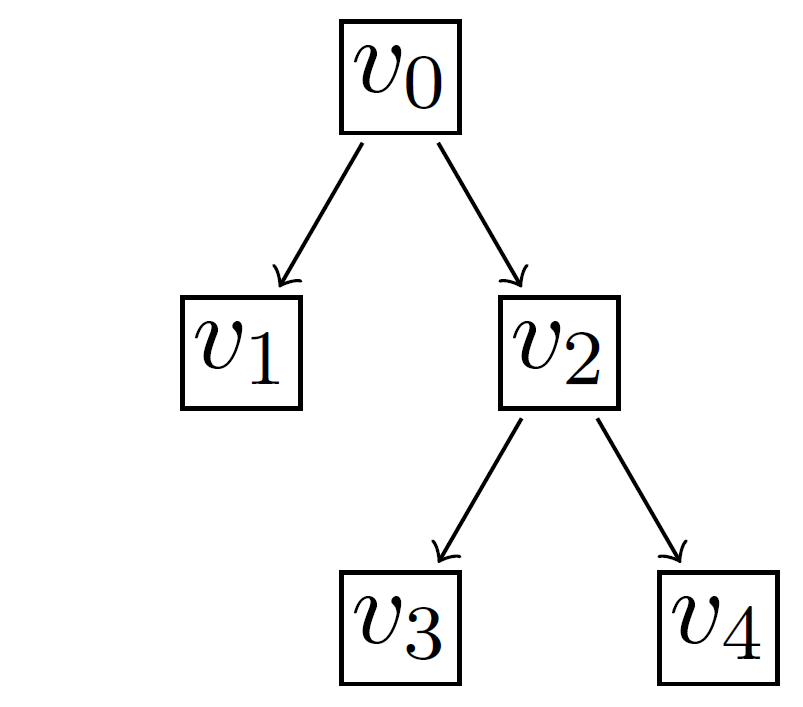
\includegraphics[scale=0.2]{pic1}
\end{center}
\begin{center}
	Рис. 1. дерево решений
\end{center}
\subsection{Бинарное дерево}

Дерево называется бинарным, если из любой его внутренней вершины выходит ровно два ребра. Выходящие ребра связывают каждую вершину $v$ с левой дочерней вершиной $L_v$ и правой дочерней вершиной $R_v$.
\begin{center}
	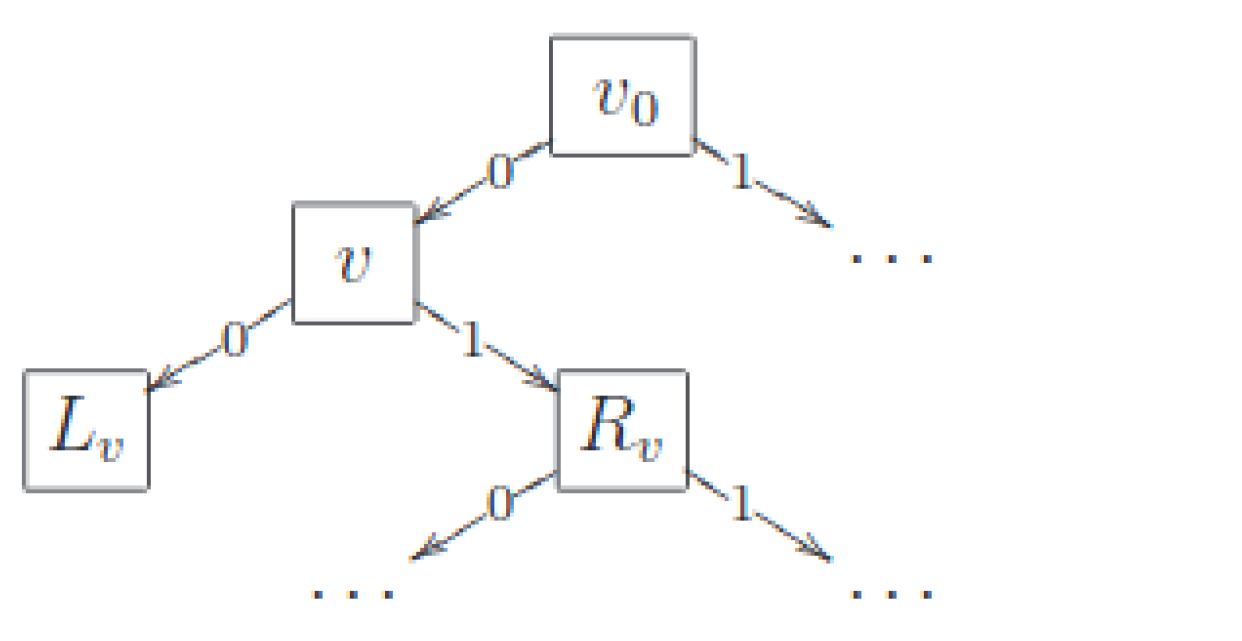
\includegraphics[scale=0.2]{pic2}
\end{center}
\begin{center}
	Рис. 2. построение бинарного дерева решений
\end{center}
\subsection{Постановка задачи}

Деревья решений применяются для классификации и регрессии. Пусть $\textbf{X}$ --- множество объектов, $\textbf{y}$ --- множество ответов. 

Если $\textbf{y}$ --- бинарный или номинальный признак, то решаем задачу классификации.

Если $\textbf{y}$ --- количественный признак, то решаем задачу регрессии.

\newpage

\section{Дано}

\noindent Набор данных
$$\textbf{X} \in \mathbb{R}^{n \times p}.$$
Зависимые переменные
$$\textbf{y} \in \mathbb{R}^n.$$

\noindent $\textbf{x}_i \in \mathbb{R}^p$ --- вектор--строки $\textbf{X}$.\\
$X_j \in \mathbb{R}^n$ --- вектор--столбцы $\textbf{X}.$\\

\noindent$y \in \{1, \cdots, K \}$ --- задача классификации.\\
$y \in \mathbb{R}$ --- задача регрессии.\\

\newpage

\section{Вероятностная постановка}

\subsection{Генеральная постановка}

Предполагаем, что $\eta$ и $\bm{\xi}$ функционально зависимы:
\begin{equation}
	\eta = \varphi(\bm{\xi}) + \varepsilon,
\end{equation}
$\varphi$ --- неизвестная функция.\\
$\eta \in \mathbb{R}$ --- случайная величина, зависимая переменная.\\
$\bm{\xi} \in \mathbb{R}^p$ --- случайный вектор, признаки.\\
$\varepsilon \in \mathbb{R}$ --- случайная величина, ошибка.\\

\subsection{Выборочная постановка}

\begin{equation}
	y_i = \varphi(\textbf{x}_i) + \varepsilon_i,
\end{equation}
\noindent$\varphi$ --- неизвестная функция.\\
$y_i$ --- реализация случайной величины $\eta$, зависимая переменная.\\
$\textbf{x}_i$ --- реализация случайного вектора $\bm{\xi}$, признаки.\\
$\varepsilon_i \in \mathbb{R}$ --- реализация случайной величины $\varepsilon$, ошибка.\\

\newpage

\section{Регрессионные деревья}
Идея построения дерева решений заключается в разделении пространства признаков $X_1, \cdots, X_p$ на $J$ непересекающиеся области $R_1, \cdots, R_J$.\\

\noindent \textbf{Модель}
\begin{equation}
	\varphi(\textbf{x}_i, \bm{\Theta}) = \sum\limits_{j=1}^{J} c_j \mathbb{I}_{(\textbf{x}_i \in R_j)}.
\end{equation}
$\textbf{x}_i \in \mathbb{R}^p$ --- индивиды.\\
$\bm{\Theta} \in \mathbb{R}^p$ --- вектор коэффициентов.\\
$\bm{\Theta} = \{ c_1, \cdots, c_J \}$.\\
$\mathbb{I}_{(\textbf{x}_i \in R_j)}$ --- индикаторная функция принадлежности индивида $\textbf{x}_i$ области $R_j$.\\

\noindent\textbf{Функция потерь}
\begin{equation}
	\text{RSS} = \sum\limits_{j=1}^{J} \sum\limits_{\textbf{x}_i \in R_j}^{} (y_i - \varphi(\textbf{x}_i, \bm{\Theta}))^2.
\end{equation}
\textbf{Оптимизация}
\begin{equation}
	\text{RSS} = \sum\limits_{j=1}^{J} \sum\limits_{\textbf{x}_i \in R_j}^{} (y_i - \varphi(\textbf{x}_i, \bm{\Theta}))^2 \to \underset{R_1, \cdots, R_J}{\min}.
\end{equation}
Тогда
\begin{equation}
	\hat{c}_j = \dfrac{1}{|R_j|} \sum\limits_{\textbf{x}_i \in R_j} y_i.
\end{equation}

\newpage

\subsection{Пример регрессии}

\begin{center}
	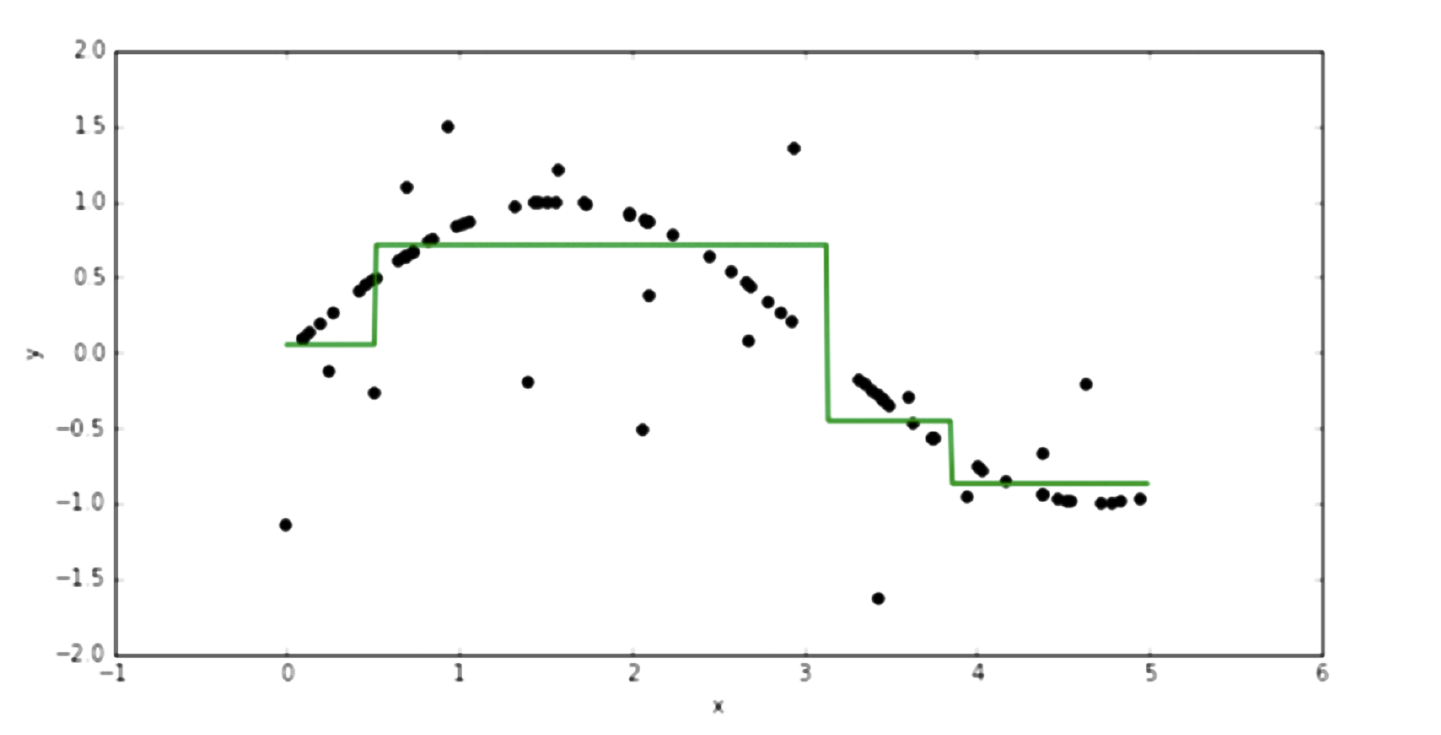
\includegraphics[scale=0.4]{pic31}
\end{center}
\begin{center}
	Рис. 3. модель регрессионного дерева решений
\end{center}
\begin{center}
	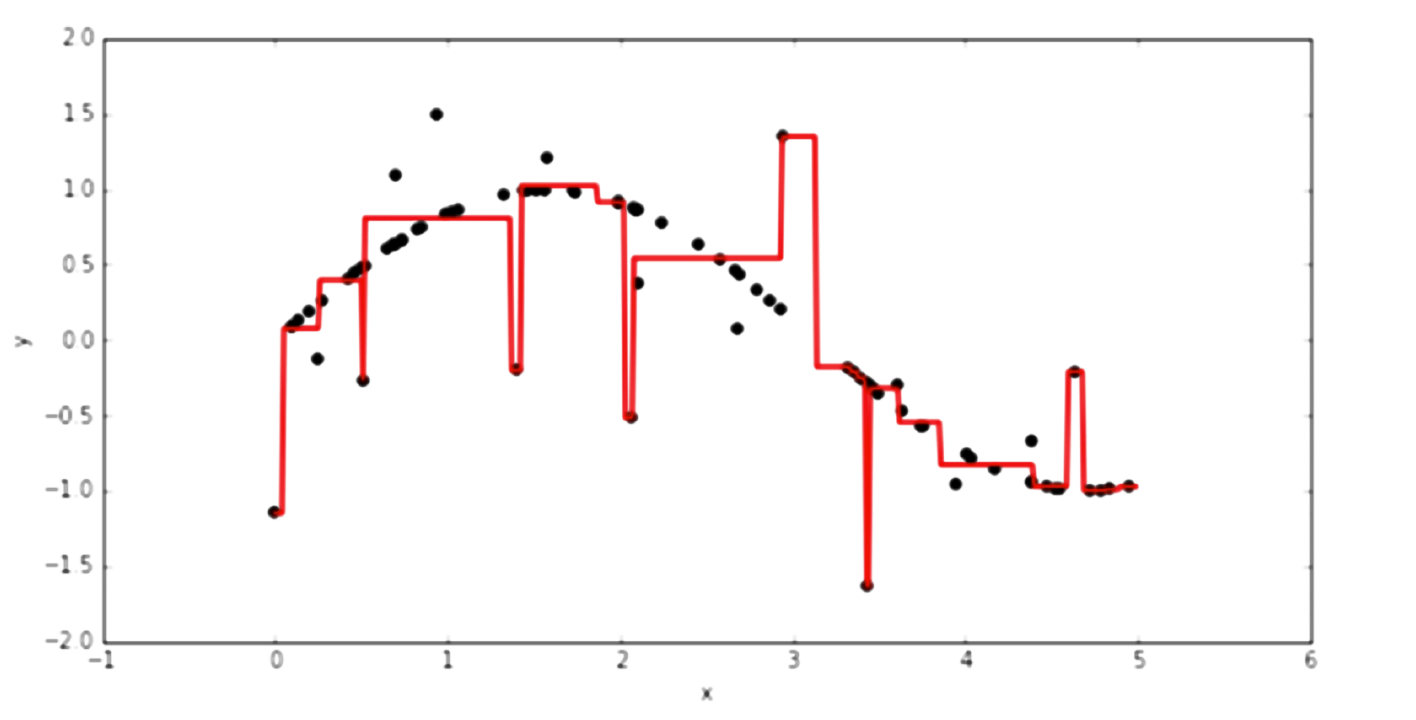
\includegraphics[scale=0.4]{pic32}
\end{center}
\begin{center}
	Рис. 4. модель переобученного регрессионного дерева решений
\end{center}

\newpage

\begin{center}
	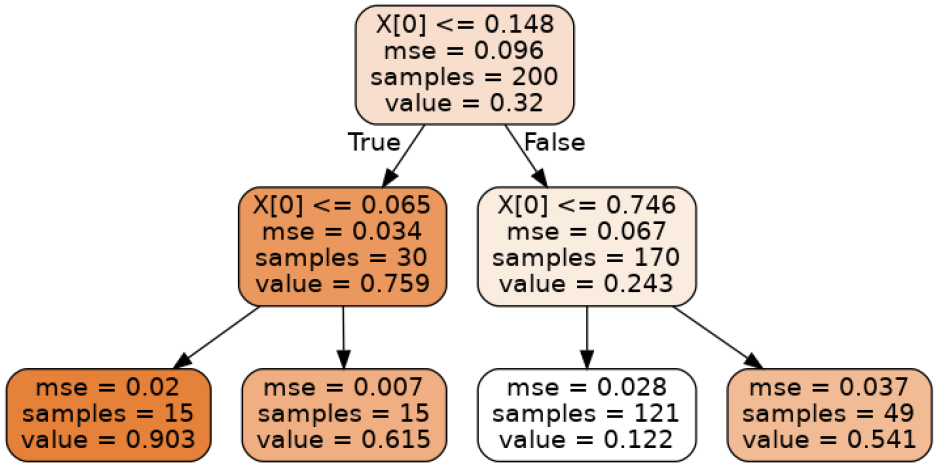
\includegraphics[scale=0.4]{pic101}
\end{center}
\begin{center}
	Рис. 5. регрессионное дерево решений
\end{center}
\begin{center}
	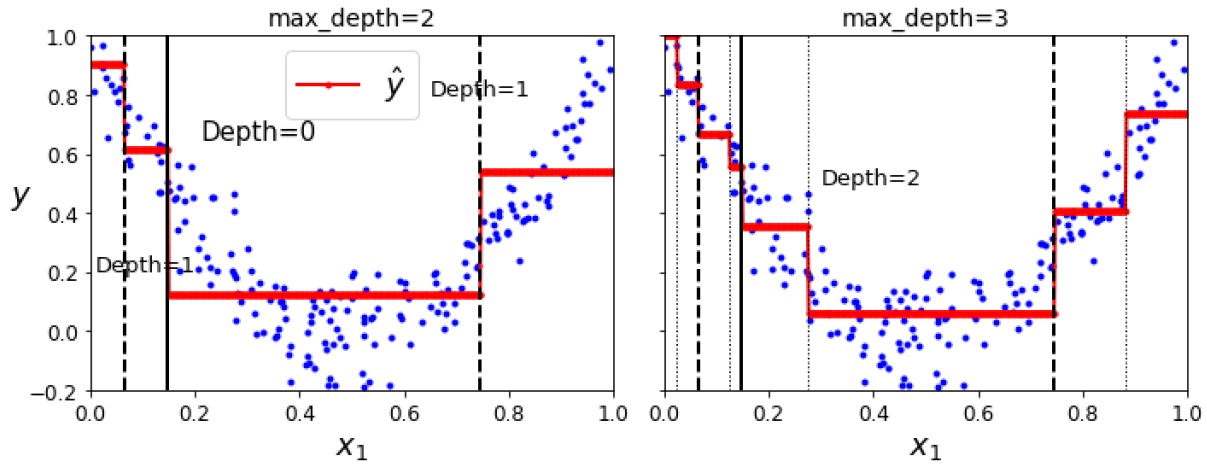
\includegraphics[scale=0.5]{pic102}
\end{center}
\begin{center}
	Рис. 6. модели регрессионного дерева решений
\end{center}


\newpage

\section{Классификационные деревья}
\noindent \textbf{Модель}\\
\begin{equation}
	\varphi(\textbf{x}_i, \bm{\Theta}) = \sum\limits_{j=1}^{J} c_j \mathbb{I}_{(\textbf{x}_i \in R_j)}.
\end{equation}
\noindent\textbf{Функция потерь}\\

\noindent Обозначим через ${p}_{jk}$ долю тренировочных индивидов в области $R_j$ из класса $k \in \{ 1, \cdots, K \}$
\begin{equation}
	{p}_{jk} = \dfrac{1}{|R_j|} \sum\limits_{\textbf{x}_i \in R_j} \mathbb{I}_{(y_i = k)}.
\end{equation}

\subsubsection{Частота ошибок классификации}

Естественной альтернативой RSS является частота ошибок классификации. это просто часть обучающих наблюдений в этой области, которые не принадлежат к наиболее распространенному классу:

\begin{equation}
	E = \dfrac{1}{|R_j|} \sum\limits_{\textbf{x}_i \in R_j}^{} \mathbb{I}_{(y_i \neq k)}.
\end{equation}

\subsubsection{Индекс Джинни}

Интерпретация: Индекс Джинни является показателем того, как часто случайно выбранный элемент будет классифицировать неверно.

\begin{equation}
	G = \sum\limits_{k=1}^{K} {p}_{jk}(1-{p}_{jk}).
\end{equation}
Индекс Джинни узла измеряет его загрязненность. Узел "чист" ($G = 0$) если все обучающие образцы, к которым он применяется, принадлежат одному и тому же классу.

\begin{center}
	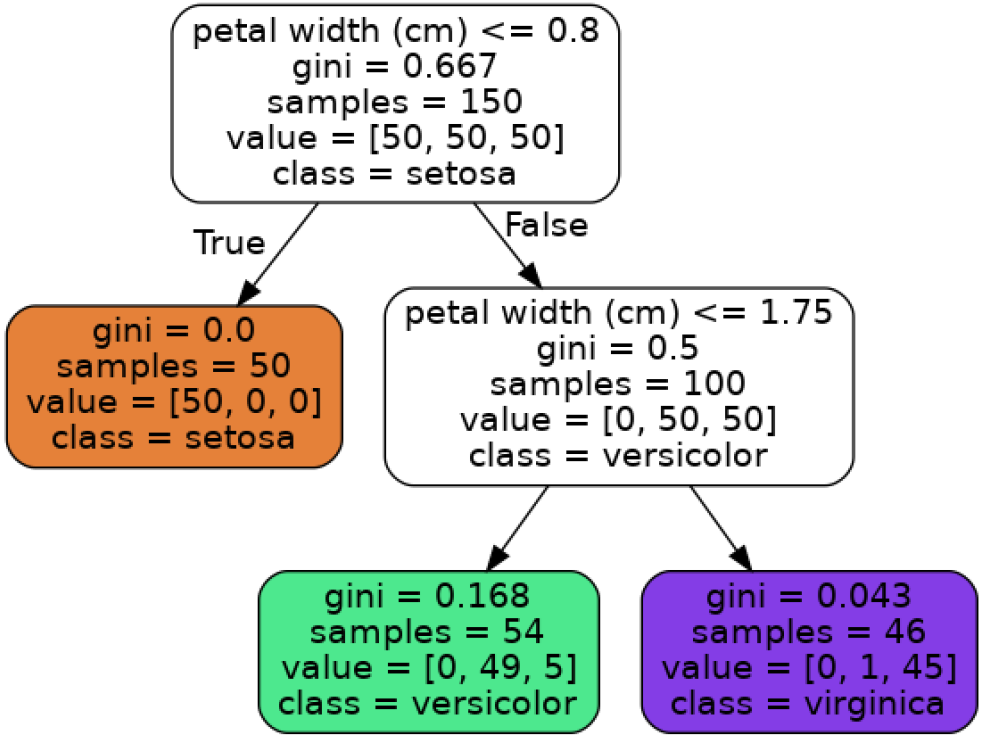
\includegraphics[scale=0.5]{piciris}
\end{center}
\begin{center}
	Рис. 7. дерево решений
\end{center}

Рассмотрим, как подсчитывается показатель Джини $G_i$ для $i$-го узла
$$G = \sum\limits_{k=1}^{K} {p}_{jk}(1-{p}_{jk}),$$
$$G = 1 - \sum\limits_{k=1}^{K} p_{jk}^2,$$
где $p_{jk}$ --- доля образцов класса $k$ среди обучающих образцов в $i$-ом узле.\\

Узел на глубине 0 имеет Индекс Джини
$$1 - \left(\dfrac{50}{150} \right)^2 - \left(\dfrac{50}{150} \right)^2 - \left(\dfrac{50}{150} \right)^2 = 1 - 3 \cdot \left(\dfrac{1}{3} \right)^2 = 1 - \dfrac{1}{3} = 0.666. $$ 
Загрязненность $G = 0.666$, т.к. 50 индивидов неверно отнесены к \textit{versicolor} и 50 неверно отнесены к \textit{virginica}.\\

Узел на глубине 1 слева имеет Индекс Джини
$$1 - \left( \dfrac{50}{50} \right)^2 - 0 - 0 = 0.$$
Загрязненность $G = 0.0$, т.к. все 50 индивидов верно отнесены к \textit{setosa}.\\

Узел на глубине 1 справа имеет Индекс Джини
$$1 - 0 - \left( \dfrac{50}{100} \right)^2 - \left( \dfrac{50}{100} \right)^2 = 0.5. $$
Загрязненность $G = 0.5$, т.к. 50 индивидов неверно классифицированы и отнесены к \textit{virginica}.\\

Узел на глубине 2 слева имеет Индекс Джини
$$1 - 0 - \left( \dfrac{49}{54} \right)^2 - \left( \dfrac{5}{54} \right)^2 = 0.168.$$
Загрязненность $G = 0.168$, т.к. 5 индивидов неверно классифицированы и отнесены к \textit{versicolor}.\\

Узел на глубине 2 справа имеет Индекс Джини
$$1 - 0 - \left( \dfrac{1}{46} \right)^2 - \left( \dfrac{45}{46} \right)^2 = 0.043.$$
Загрязненность $G = 0.043$, т.к. 1 индивид неверно классифицирован и отнесен к \textit{virginica}.

\subsubsection{Кросс-энтропия}

\begin{equation}
	CI = - \sum\limits_{k=1}^{K} {p}_{jk} \log {p}_{jk}.
\end{equation}

Интерпретация: из теории вероятностей известно, что энтропия ограничена снизу нулем, причем минимум достигается на вырожденных распределениях ($p_i = 1, pj = 0$ для $i \neq j$). Максимальное же значение энтропия принимает для равномерного распределения. Отсюда видно, что энтропийный критерий отдает предпочтение более «вырожденным» распределениям классов в вершине.

\begin{center}
	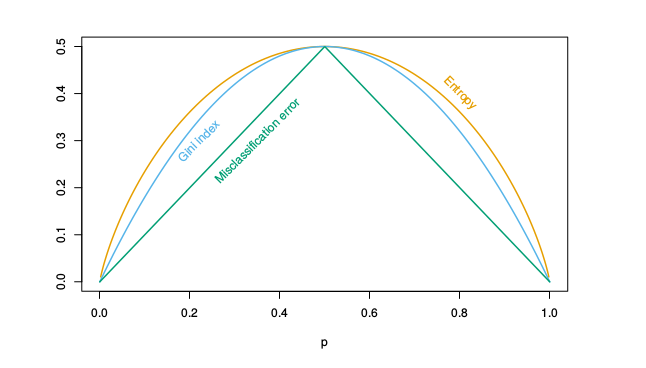
\includegraphics[scale=1]{pic5}
\end{center}
\begin{center}
	Рис. 8. Загрязненность \textit{impurity} узла для двухклассовой классификации измеряется как доля индивидов $p$, отнесенных ко второму классу
\end{center}

\newpage

\section{Алгоритмы}

\subsection{CART (использует Индекс Джини)}

\noindent Выбираем признак $X_j$ и порог $s$ так, чтобы разбиение $\textbf{X}$ на
$$R_1(j,s) = \{ \textbf{x}_i \in \textbf{X} | X_j < s \}$$
и
$$R_2(j,s) = \{ \textbf{x}_i \in \textbf{X} | X_j \geq s \}$$
решало задачу
\begin{equation}
	\sum\limits_{i:\textbf{x}_i \in R_1 (j,s)} (y_i - \hat{c}_1) + 	\sum\limits_{i:\textbf{x}_i \in R_2 (j,s)} (y_i - \hat{c}_2) \to \min_{j,s}
\end{equation}
где оценка коэффициента $\hat{c}_j = \dfrac{1}{|R_j|} \sum\limits_{\textbf{x}_i \in R_j(j,s)} y_i, \quad j = 1,2.$\\

\begin{enumerate}
	\item Перебираем все возможные $s_j$ и выбираем то значение, при котором Индекс Джини минимален.
	\item Разбиваем выборку на области $R_1$ и $R_2$, образуя две дочерние вершины $L_v$ и $R_v$.
	\item Повторяем процедуру, разбивая каждый из получившихся регионов, пока не будет достигнута максимальная глубина.
	\item Алгоритм CART --- жадный, он выбирает наилучшее расщепление на текущем уровне, что не обязательно приводит к наименьшей загрязненности на уровнях ниже. Алгоритм хорош, но не всегда оптимален.
\end{enumerate}

\subsection{ID3 (использует Кросс-энтропию)}

Идея алгоритма заключается в последовательном дроблении выборки на две части
до тех пор, пока в каждой части не окажутся объекты только одного класса. Нам необходимо выбирать такой предикат, чтобы ветвление дерева было максимально информативно

\begin{enumerate}
	\item $\textbf{X}$ --- обучающая выборка, $\textbf{y} \in \{1, \cdots, k\}$.
	\item Если все $\textbf{x}_i$ имеют класс $k$, ставим метку 1 в корень и выходим из цикла.
	\item Если ни один $\textbf{x}_i$ не имеет класс $k$, ставим метку 0 в корень и выходим из цикла.
	\item Предикат $R(\textbf{x}_i):=\{ \textbf{x}_i | X_j \lessgtr s_j \}$ для которого информационная выгода наибольшая.
	\item Разбиваем $\textbf{X}$ на $\textbf{X}_0$ и $\textbf{X}_1$ по предикату $R$
	$$\textbf{X}_0:=\{ \textbf{x}_i \in \textbf{X}:R(\textbf{x}_i) = 0 \},$$
	$$\textbf{X}_1:=\{ \textbf{x}_i \in \textbf{X}:R(\textbf{x}_i) = 1 \}.$$
	\item Если $\textbf{X}_0 = \varnothing$ или $\textbf{X}_1 = \varnothing$, создаем новый лист $v$, $k_v$ --- класс, в котором находится большинство элементов $\textbf{x}_i.$
	\item Иначе создаем внутреннюю вершину $v$:
		\begin{enumerate}
			\item $R_v = R$;
			\item $L_v$;
			\item $R_v$.
		\end{enumerate}
\end{enumerate}

\subsection{Стрижка деревьев}

Описанный выше процесс может дать хорошие прогнозы на обучающем наборе, но, вероятно, \textit{переобучится}, что приведет к плохим результатам на тестовых наборах. Почему?

Меньшее дерево с меньшим количеством разбиений (то есть с меньшим количеством областей $R_1, \cdots, R_J$) может привести к меньшей дисперсии и лучшей интерпретации за счет небольшого смещения. Мы можем пожертвовать смещением, но получить меньшую дисперсию.

Одна из возможных альтернатив описанному выше процессу --- выращивать дерево только до тех пор, пока уменьшение RSS из-за каждого разбиения превышает некоторый (высокий) порог.

Эта стратегия приведет к уменьшению размеров деревьев, но она слишком недальновидна: за кажущимся бесполезным разбиением в начале дерева может последовать очень хорошее разбиение --- то есть разделение, которое в дальнейшем приводит к значительному сокращению RSS.

Лучшая стратегия --- вырастить очень большое дерево $T_0$, а затем обрезать его, чтобы получить поддерево.

\textit{Cost complexity prunning} --- также называется сокращением наиболее слабых звеньев --- используется для этого.

Мы рассматриваем последовательность деревьев, с настраиваемыми параметрами $\alpha$. Каждому значению $\alpha$ соответствует поддерево $T \subset T_0$ (является подмножеством) такое, что
\begin{equation}
	\sum\limits_{j=1}^{|T|} \sum\limits_{\textbf{x}_i \in R_j}^{} (y_i - \hat{y}_{R_j})^2 + \alpha |T|.
\end{equation}
настолько мало насколько это возможно. Здесь $|T|$ указывает количество конечных узлов дерева $T$, $R_j$ --- это прямоугольник (\textbf{то есть подмножество пространства предикторов}), соответствующий $j$-му конечному узлу, а $\hat{y}_{R_j}$ --- это среднее значение обучающих наблюдений в $R_j$.

\textbf{Критерий остановки}:\\
1. Ограничение макс. глубины дерева;\\
2. Ограничение мин. числа объектов в листе $n_{min}$;\\
3. Ограничение макс. количества листьев в дереве;\\
4. Остановка в случае, если все объекты в листе относятся к одному классу.

\newpage

\subsection{Пример классификации: данные о бейсболе}

Рассмотрим данные о зарплате в бейсболе. Заработная плата имеет цветовую маркировку от низкой (синий, зеленый) до высокой (желтый, красный).

Для данных \textbf{Hitters} - дерево регрессии для прогнозирования логарифма зарплаты бейсболиста на основе количества лет, которые он играл в высшей лиге, и количества попаданий, сделанных им в предыдущем году.

В данном внутреннем узле метка (в форме $X_j < t_k$) указывает левую ветвь, исходящую из этого разделения, а правая ветвь соответствует $X_j \geq t_k$. Например, разделение на вершине дерева приводит к образованию двух больших ветвей. Левая ветвь соответствует $Years < 4.5$, а правая ветвь соответствует $Years \geq 4.5$.

Дерево имеет два внутренних узла и три конечных узла, или три листа. Число на каждом листе --- это среднее значение отклика на попадающие туда наблюдения.

В итоге, дерево разбивает или сегментирует игроков на три области пространства предикторов:
$$R_1 = \{ X | Years < 4.5 \},$$
$$R_2 = \{ X | Years \geq 4.5, Hits < 117.5 \},$$
$$R_3 = \{ X | Years \geq 4.5, Hits \geq 117.5 \}.$$
\begin{center}
	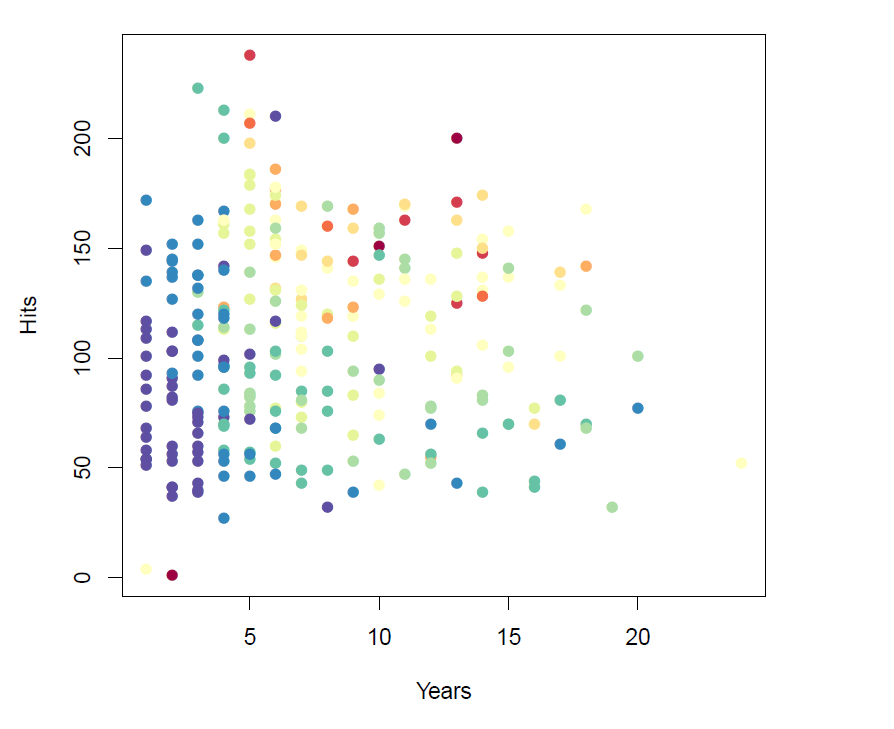
\includegraphics[scale=0.3]{pic61}
\end{center}
\begin{center}
	Рис. 9. данные о бейсболе
\end{center}
\begin{center}
	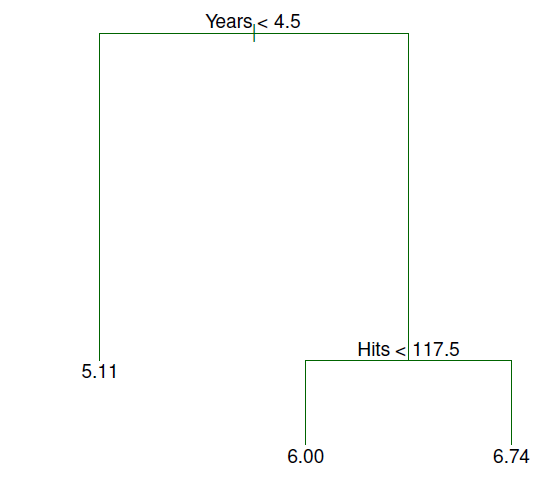
\includegraphics[scale=0.4]{pic62}
\end{center}
\begin{center}
	Рис. 10. классификационное дерево
\end{center}
\begin{center}
	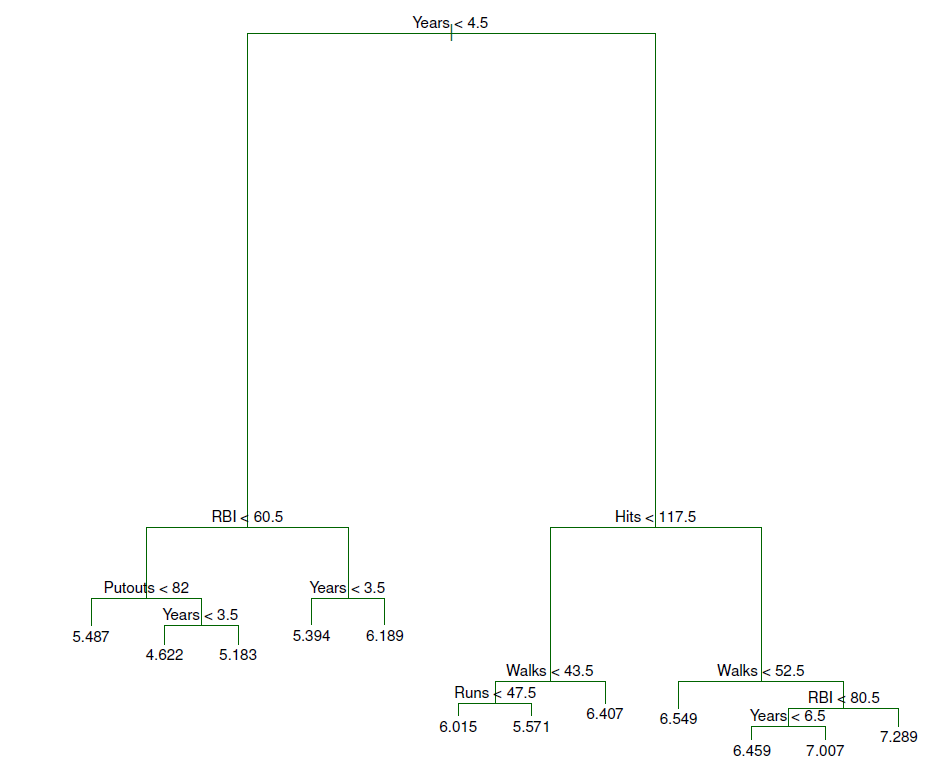
\includegraphics[scale=0.3]{pic63}
\end{center}
\begin{center}
	Рис. 11. переобученное классификационное дерево
\end{center}
\begin{center}
	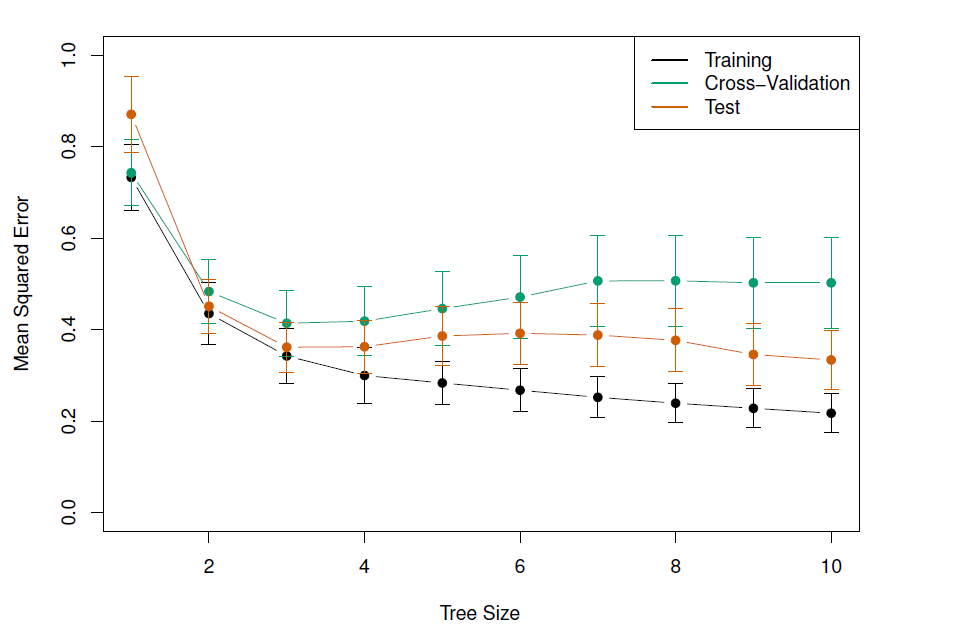
\includegraphics[scale=0.3]{pic64}
\end{center}
\begin{center}
	Рис. 12. средневквадратичная ошибка в зависимости от размера дерева
\end{center}
\begin{center}
	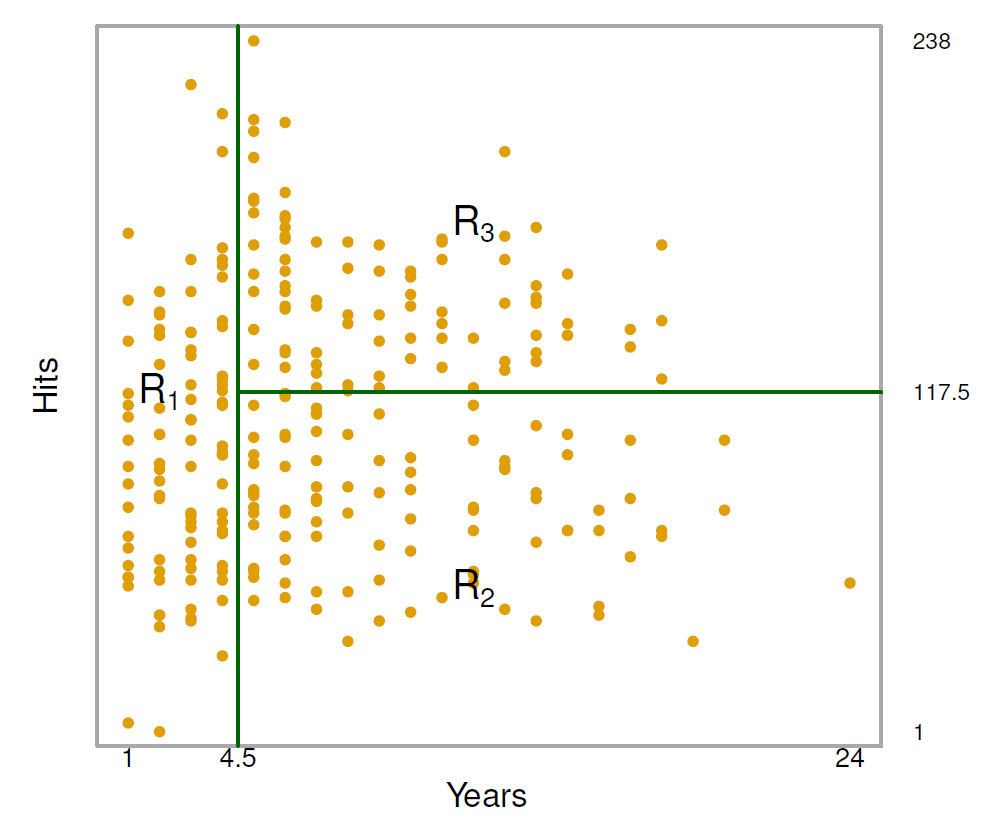
\includegraphics[scale=0.25]{pic65}
\end{center}
\begin{center}
	Рис. 13. результат классификации
\end{center}

\newpage

\subsection{Пример классификации: данные о сердце}

Эти данные содержат бинарный результат $HD$ для 303 пациентов с болью в груди.

Значение результата $Yes$ указывает на наличие сердечного заболевания на основании ангиографического теста, в то время как $No$ означает отсутствие сердечного заболевания.

Существует 13 предикторов, включая $Age, Sex, Chol$ (измерение холестерина) и другие измерения функции сердца и легких.

Перекрестная проверка дает дерево с шестью конечными узлами.

\begin{center}
	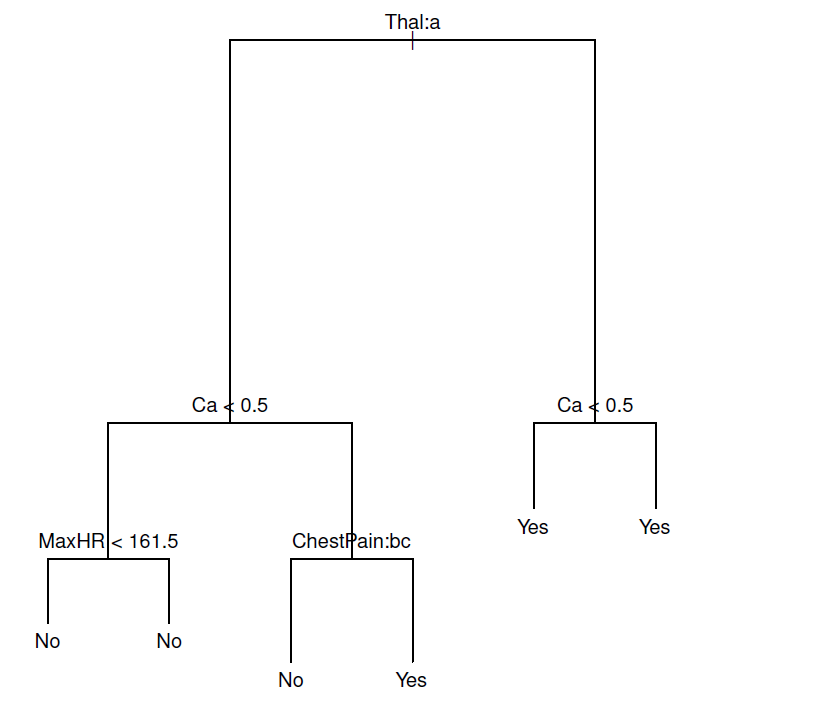
\includegraphics[scale=0.3]{pic71}
\end{center}
\begin{center}
	Рис. 14. классификационное дерево
\end{center}
\begin{center}
	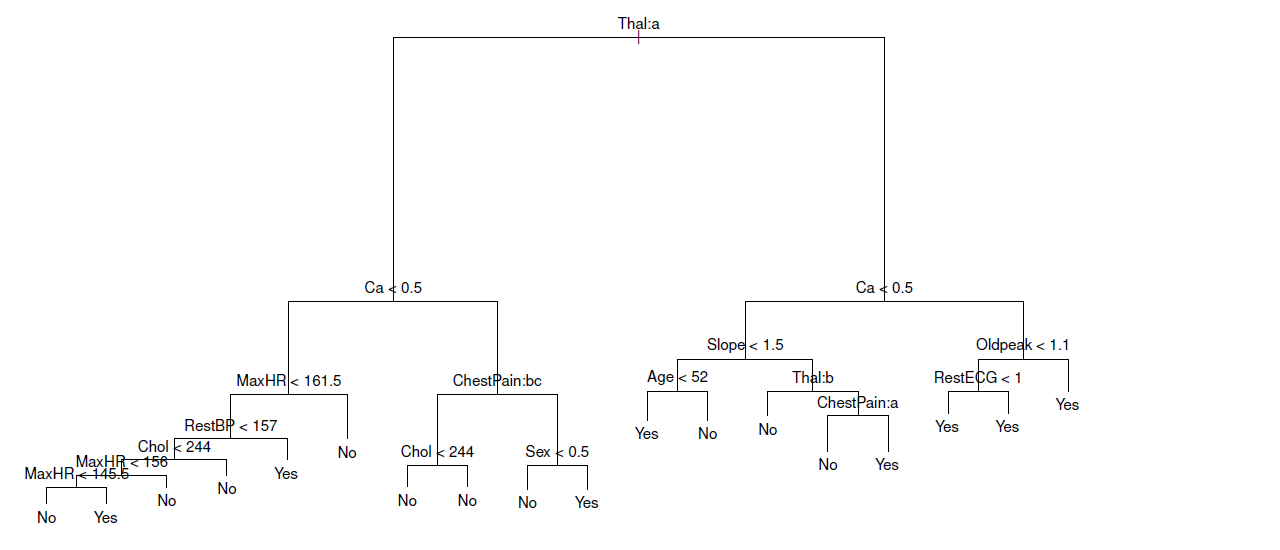
\includegraphics[scale=0.3]{pic72}
\end{center}
\begin{center}
	Рис. 15. переобученное классификационное дерево
\end{center}
\begin{center}
	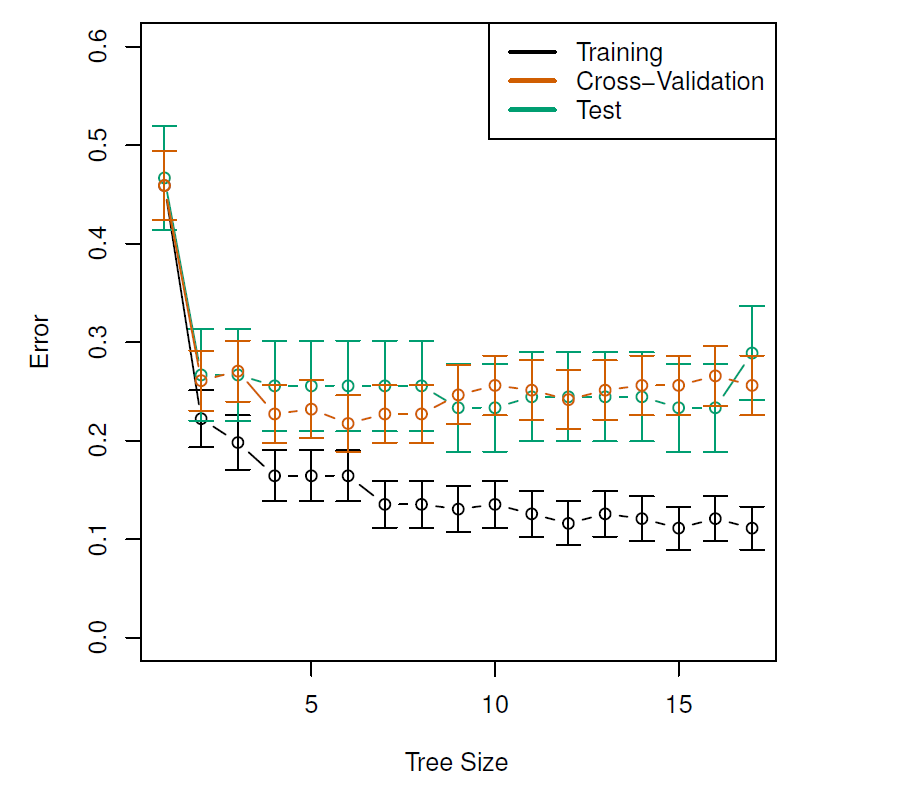
\includegraphics[scale=0.3]{pic73}
\end{center}
\begin{center}
	Рис. 16. среднеквадратичная ошибка в зависимости от размера дерева
\end{center}

\newpage

\section{Подведение итогов}

\subsection{Сравнение деревьев с линейными моделями}

\begin{center}
	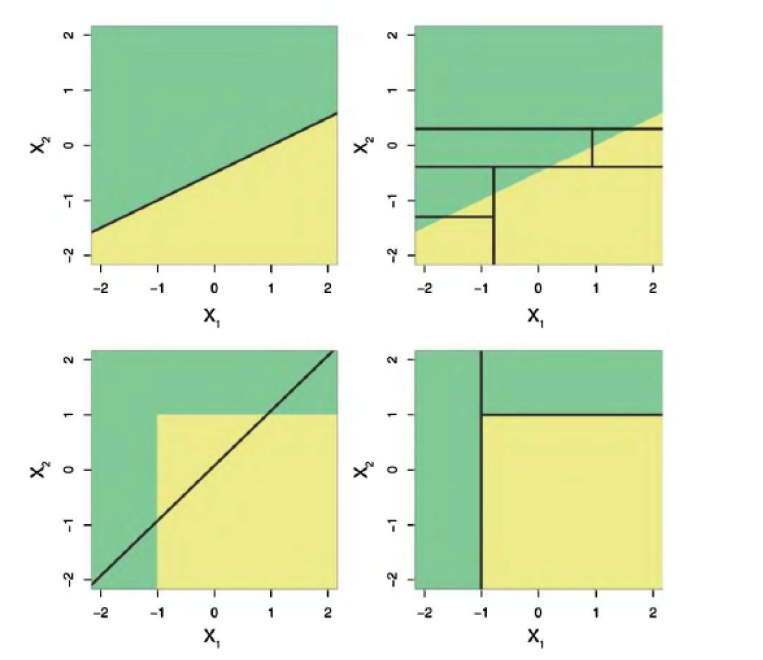
\includegraphics[scale=0.5]{pic10}
\end{center}
\begin{center}
	Рис. 17. сравнение моделей
\end{center}
\subsection{Преимущества и недостатки рещающих деревьев}

\textbf{Преимущества}:\\
1. Пригодность для задач как классификации, так и регрессии.\\
2. Легко визуализировать.\\
3. Легко интерпретировать.\\
4. Деревья отражают процесс принятия решения человеком.

\textbf{Недостатки}:\\
1. Невысокая точность.\\
2. Склонность к переобучению.

\end{document}